\chapter{\IfLanguageName{dutch}{Vaktermen binnen een First Person Shooter}{Vaktermen binnen een First Person Shooter}}
\label{ch:Vaktermen-binnen-een-First-Person-Shooter}

\section{Algemene introductie}
Een \textit{First Person Shooter} bestaat uit verschillende systemen en modules die samen zorgen voor de volledige spelervaring. Binnen een FPS bestuurt de speler een personage vanuit het eerstepersoonsperspectief, vandaar ook de naam ``first person''.

\section{Game engine}
De basis van een FPS-game wordt gevormd door de \textit{game engine}. Een game engine is de softwarelaag die verantwoordelijk is voor graphics, physics, geluiden, animaties en de algemene verwerking van het spel. Bekende voorbeelden hiervan zijn Unreal Engine en Unity.

\section{Game control system}
Daarnaast beschikt een FPS-game over een \textit{game control system}. Dit systeem vormt de laag die alle input van de speler interpreteert en vertaalt naar acties binnen het spel. Elke actie die een speler uitvoert via een Human Interface Device, zoals een toetsenbord, muis of controller, wordt eerst verwerkt door dit systeem voordat ze invloed heeft op de spelwereld.
\\\\
Het game control system bepaalt onder andere de bewegingslogica van het personage, zoals lopen, sprinten, springen en bukken. Hierbij wordt niet enkel gekeken naar binaire input (bijvoorbeeld een toets die ingedrukt wordt), maar ook naar parameters zoals snelheid, versnelling en vertraging naar gelang jouw voorkeur.
\\\\
Daarnaast wordt ook de camerabesturing binnen dit systeem afgehandeld. De beweging van de muis of analoge stick wordt omgezet naar rotaties in het videospel zoals rondkijken, waarbij meestal gebruik wordt gemaakt van een gevoeligheidsinstelling (sensitivity) en soms ook acceleratiecurves. Hierdoor kan dezelfde input een verschillend effect hebben afhankelijk van de ingestelde parameters.
\\\\
Dit systeem is doorgaans configureerbaar via de instellingen van de game, waar spelers hun besturingsschema en gevoeligheid kunnen aanpassen naar persoonlijke voorkeur.

\begin{figure}[H]
    \centering
    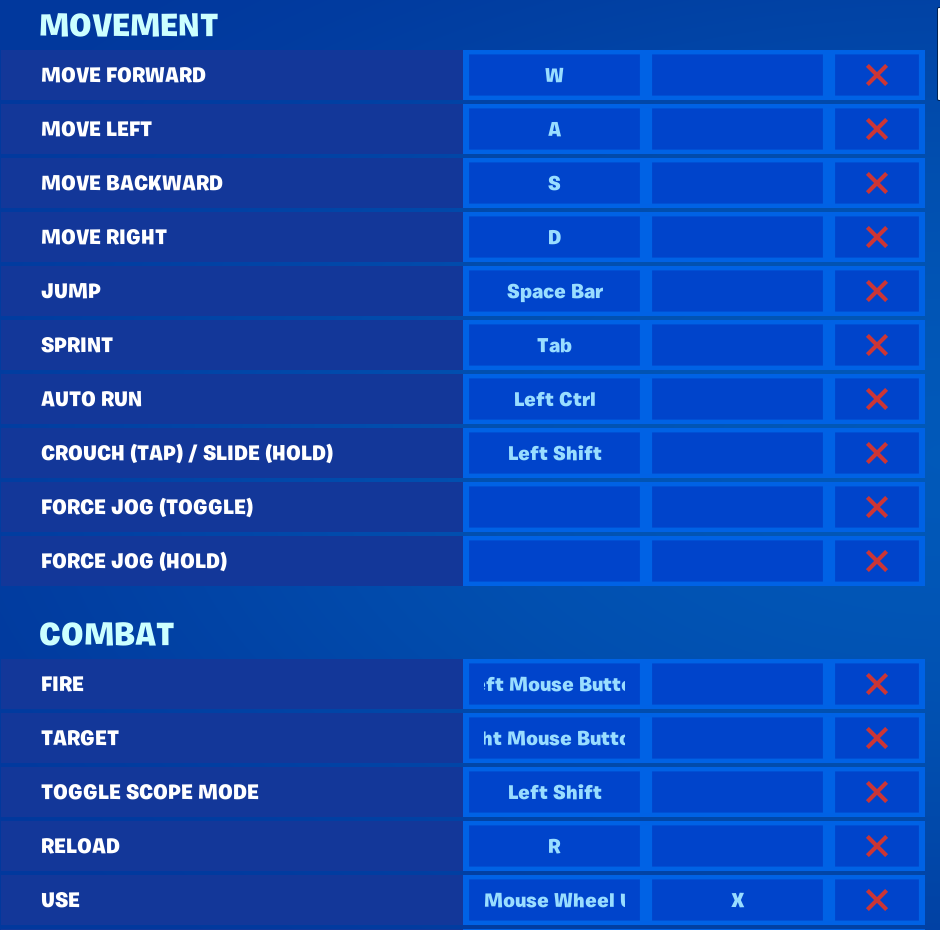
\includegraphics[height=6cm]{../fotos/instellingen.png}
    \caption{Voorbeeld van toetsenbordinstellingen van Fortnite Battle Royale}
    \label{fig:instellingen}
\end{figure}

\section{Human Interface Devices (HID)}
De besturing van een FPS-game gebeurt via \textit{Human Interface Devices} (HID's). Dit zijn randapparaten die ontworpen zijn om gebruikersinput rechtstreeks naar een computersysteem te verzenden via gestandaardiseerde communicatieprotocollen, zoals USB HID. Het besturingssysteem herkent deze apparaten als invoerbronnen en vertaalt de ontvangen signalen naar digitale inputevents binnen de game-engine.
\\\\
HID's genereren inputrapporten die onder andere informatie bevatten over toetsdrukken, muisbewegingen, analoge stickposities en knopstatussen. Deze rapporten worden op regelmatige tijdsintervallen verstuurd naar het systeem, waar ze worden verwerkt door de inputlaag van het besturingssysteem en vervolgens doorgestuurd naar de applicatielaag van de game.
\\\\
\newpage
Voorbeelden van dergelijke apparaten zijn toetsenborden, computermuizen en gamecontrollers.

\begin{figure}[H]
    \centering
    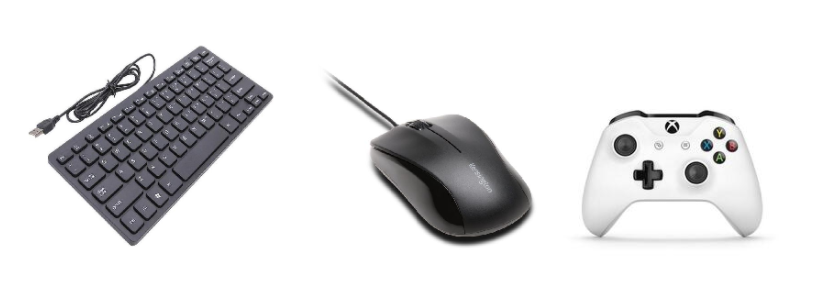
\includegraphics[width=0.8\textwidth]{../fotos/hid_apparaten.png}
    \caption{Voorbeelden van Human Interface Devices (HID's)}
    \label{fig:hid-apparaten}
\end{figure}

\section{HUD (Heads-Up Display)}
Verder bevat een FPS-game meestal een \textit{HUD} of \textit{Heads-Up Display}. Dit is de gebruikersinterface die vaak informatie toont zoals gezondheid, munitie, minimap en score-informatie.

\begin{figure}[H]
    \centering
    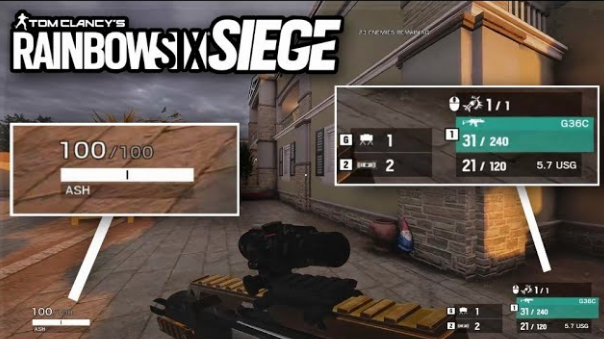
\includegraphics[width=0.8\textwidth]{../fotos/HUD.png}
    \caption{Voorbeeld van de HUD uit Tom Clancy's Rainbow Six Siege}
    \label{fig:HUD}
\end{figure}

\section{Relevantie voor deze bachelorproef}
Omdat moderne cheats zich vaak richten op geautomatiseerde aiming en recoilcompensatie, vormt vooral het recoilmechanisme een belangrijk onderdeel binnen deze bachelorproef.